\subsection{Architecture}

The only dependencies used are JUnit and JUnit-jupiter \cite{junit} for testing purposes.

The following figure illustrates the architecture and design of the \verb|gp-modifiable-ast| library.
Each small rectangle represents an entity of the entire program, the small rectangles with \textbf{bold} text are user-defined inputs and implementations and
the ones with \textit{italic} text are implementations of the \verb|gp-modifiable-ast| library.


\begin{figure}[H]
    \centering
    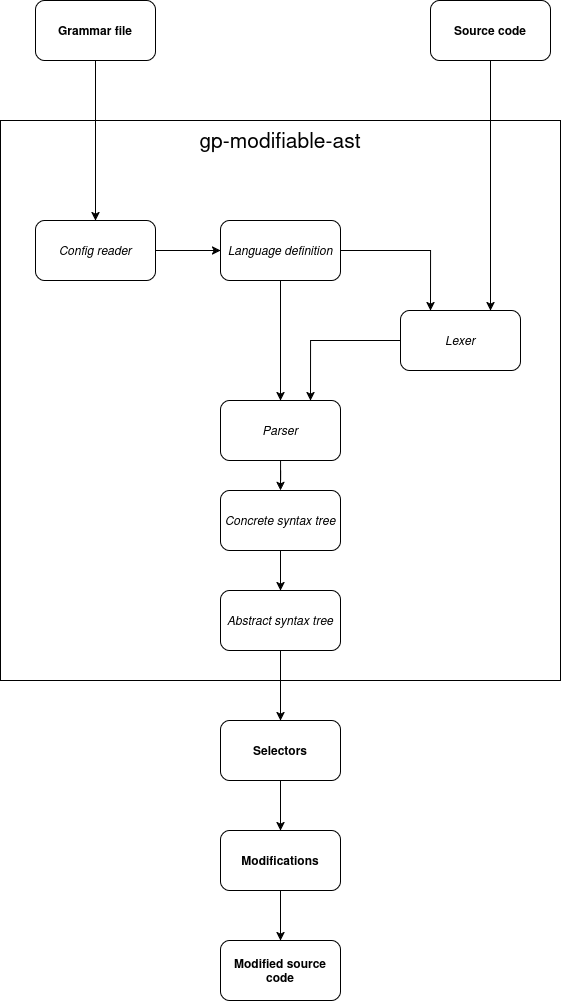
\includegraphics[scale=0.40]{fig/architecture.png}
    \caption{Architecture of gp-modifiable-ast}
\end{figure}

The user defines a grammar file for a given programming language and provides the source code to \verb|gp-modifiable-ast|.

\verb|gp-modifiable-ast| first parses the grammar file and creates a language definition that contains the grammar productions, lexer rules, and generic settings for the language.

This language definition is then passed along with the source code by the user to the lexer process, 
which passes the token stream and the language definition to the
to the parser process. The parser process parses the token stream, applies the grammar rules and creates the concrete syntax tree.

In the next step, the concrete syntax tree and the grammar definition will be used to create the abstract syntax tree.

This is the output of the \verb|gp-modifiable-ast| library. By using selectors, which will be defined later, 
the user can perform search actions on the AST to find
specific nodes. On the nodes found, the user can apply modifications and convert the AST back to source code.

